\documentclass[]{UCD_CS_FYP_Report}
\usepackage{graphicx}
\usepackage{listings}
\usepackage{hyperref}
\hypersetup{
    colorlinks=true,
    linkcolor=blue,
    filecolor=magenta,      
    urlcolor=cyan,
}
\lstset{
    mathescape=true,
    basicstyle = \ttfamily
}
%\usepackage[backend=biber,style=chicago-authordate]{biblatex}
\usepackage[backend=biber,style=nature]{biblatex}
\addbibresource{references.bib}


%%%%%%%%%%%%%%%%%%%%%%
%%% Input project details

\def\studentname{Sabeer Bakir}% Edit with your name
\def\studentid{16333886}% Edit with your student id
\def\projecttitle{Learning shortest path tours to all pubs in UK} % Edit with you project title
\def\supervisorname{Deepak Ajwani}


\begin{document}
\maketitle

%%%%%%%%%%%%%%%%%%%%%%
%%% Table of Content

\tableofcontents
%\pdfbookmark[0]{Table of Contents}{toc}\newpage
%\newpage


%%%%%%%%%%%%%%%%%%%%%%
%%% Your Abstract here
\abstract
Designing algorithms for NP-hard combinatorial optimization problems over graphs is a complex task. It has been shown with use of good heuristics and approximation algorithms that these problems can be solved in polynomial time. However, these solutions require problem-specific knowledge and trial-and-error. Is it possible to automate this learning process with the use of machine learning classification? In real world applications, the data is very rarely similar however the structures within may not differ as much. In this paper, we will explore a method to solve the Travelling Salesman Problem (TSP) using classification to identify edges that are contained within the tour created by the TSP. The applications of this can be applied in many areas such as, DNA Sequencing, Route Planning, Logistics Management, etc.


%%%%%%%%
\chapter{Project Specification}
\LARGE Core
\normalsize
\begin{itemize}
    \item Identify features of edges that can discriminate between edges in the shortest TSP tour and edges that are not.
    \item Take random samples of the pub crawl dataset and use a state-of-the-art heuristic on that to get the ground truth for training
    \item Use the identified features and the ground truth on random samples to train a classification model that learns the edges in the shortest TSP tour
    \item Evaluate the accuracy of the classification model
\end{itemize}
\LARGE Advanced
\normalsize
\begin{itemize}
    \item Compare the running time vs. optimality trade-off of the learning approach with the Concorde TSP solver (\url{http://www.math.uwaterloo.ca/tsp/concorde.html})
    \item Improve the accuracy of the classification algorithm by careful feature selection
\end{itemize}


%%%%%%%%
\chapter{Introduction}
The Travelling salesman problem (TSP) is a combinatorial graph optimization question that is. This problem is NP-hard and has caused considerable interest by theory and algorithm design communities in the past. In the realm of computational complexity, one of Karp's 21 NP-complete problems is the Hamiltonian Cycle Problem, this is a special case of the travelling salesman problem.\\[0.2cm] 
The TSP was first introduced in the 1800s by the Irish mathematician Sir William Rowan Hamilton and the British mathematician Thomas Penyngton Kirkman. However, optimisation of the TSP only came about in the 1930s from Karl Menger in Vienna and Harvard. Menger defined the problem as, “Given a finite number of points, with known pairwise distances, find the shortest path connecting the points.”\cite{Menger}\\[0.2cm]
Techniques that are used to solve these graph optimisation problems comes in three main type: exact algorithms, approximation algorithms and heuristics. Exact algorithms always find the most optimal solution however it requires exponential time which does not scale well for large inputs. Approximation algorithms offer the desirable polynomial time solution however it is hard to guarantee the optimality for certain problems. Heuristics are typically fast but require problem specific research and experimenting from the algorithm designers.\\[0.2cm]
Designing algorithms for NP-hard combinatorial optimization problems is a complex task. It has been shown with use of good heuristics and approximation algorithms that these problems can be solved in polynomial time. However, these solutions require problem-specific knowledge and trial-and-error. Is it possible to automate this learning process with the use of machine learning classification? In real world applications, the data is very rarely similar however the structures within the data do not differ. In this paper, we will explore a method to solve the Travelling Salesman Problem (TSP) using classification to identify edges that are contained within the tour created by the TSP. We will see if it is possible to learn the shortest path to all pubs in the UK. The applications of this can be applied in many areas such as, DNA Sequencing, Route Planning, Logistics Management, etc.

%%%%%%%%
\chapter{Related Work and Ideas}
\textbf{Exact Algorithms}
An exact algorithm in the domain of optimization refers to a method that will always yield the most optimal solution. Such algorithms do exist for the TSP \cite{Bellman:1962:DPT:321105.321111}, this is one of the earliest adoptions of \textit{Dynamic Programming}. The main disadvantage to this algorithm is its runtime of $\mathcal{O}(N^22^N)$. Due to this, algorithm designers have looked towards other methods of optimisation such as heuristics and approximation algorithms.\\[0.5cm]
\textbf{Constructive Heuristics}
This approach differs from local search heuristics where a solution is given and optimality is obtained by making local changes at various points in the solution. Constructive heuristics begin with an empty solution and attempt local optimizations at each point in the solution. In \cite{JohnMcGe97}, algorithms such as \textit{Nearest Neighbour (NN)}, \textit{Greedy}, \textit{Clarke-Wright}, and
\textit{Christofides} are applied to the TSP. 
\begin{itemize}
  \item \textbf{Nearest Neighbour (NN): }This algorithm constructs a tour from starting at some arbitrary node and builds the cycle by adding the nearest neighbour from the current node. It's runtime is $\mathcal{O}(N^2)$. This provides a decent approximation for the most optimal, on average the path length is roughly 25\% longer than the most optimal path.
  \item \textbf{Greedy: }Often mistaken for Nearest Neighbour, it is constructed by taking the complete graph of the TSP instance, and the path starts with the shortest edge. It is further built by continuously adding the next shortest incident edge such that no node has degree greater than 2 or cycle length less than the total number of nodes. Its runtime is slightly longer than that of NN at $\mathcal{O}(N^2logN)$ however the worst case solution is better than NN.
  \item \textbf{Clarke-Wright (CW): }This algorithm originally comes from a vehicle routing method designed by Clarke and Write\cite{Clarke:1964:SVC:2769344.2769349}. In terms of the TSP, an arbitrary city is chosen as a central point for which the salesman would return to after each visit to another city. A \textit{savings} metric is defined as how much shorter the tour becomes if the salesman skips returning to the central point. A greedy approach is then utilized on these savings values rather than the edge distances. Since this is a different approach of the greedy algorithm, it's runtime is similarly $\mathcal{O}(N^2logN)$. This method has a higher best performance in comparison to the greedy algorithm however it's worse case performance is the same.
  \item \textbf{Christofides: }The Christofides algorithm is an approximation algorithm that ensures solutions that will be within a factor of 3/2 of the optimal solution. The tour is generated by constructing the minimum weight spanning tree where the weights are the distances between the nodes. Compute a perfect matching on the nodes of odd degree and combine with the spanning tree. This will result in a connected graph with each node having even degree. On one hand, this approach has the best worst-case solution of the constructive heuristics, on the other hand it's runtime is substantially longer than the other constructive heuristics due to the perfect matching algorithm complexity.
\end{itemize}


\textbf{Concorde TSP Solver}
In the 1990s, a collection of heuristics and functions have been designed by Applegate, Bixby, Chvátal, and Cook \cite{davidapplegate2007}. This solver holds the most records for solving large TSP instances with minuscule loss in accuracy. This precision does come at the cost of time, many large TSP problems take over 100-years of CPU time which isn't ideal for applications that require solutions to be obtained swiftly. The applications of the Concorde include: gene-mapping\cite{10.1093/jhered/esg012}, protein function prediction\cite{Johnson2006}, vehicle routing\cite{ApplegateVPR}, etc. According to \cite{MULDER2003827}, the Concorde “is widely regarded as the fastest TSP solver, for large instances, currently in existence.”\\[0.5cm]
\textbf{Reinforcement learning for Combinatorial optimization}
Reinforcement learning (RL) is used as a natural framework for learning the evaluation function in \cite{DBLP:journals/corr/DaiKZDS17}. An \textit{off-policy} RL algorithm such as Q-Learning was utilized here which updates its rules on the Q-Value rather than looking at past examples to learn. This technique was used over graph problems such as: Minimum Vertex Cut (MVC), Maximum Cut (MAXCUT), and the Travelling Salesman Problem (TSP). This type of approach lends itself to designing greedy heuristics for difficult combinatorial optimization problems. Heuristics as we know are commonly fast but in the area of optimization require certain knowledge about the underlying problem, this approach attempts to build these heuristics whilst learning about the underlying problem.\\[0.5cm]
\textbf{Deep reinforcement learning}
The use of an \textit{on-policy} technique using neural networks was applied in \cite{DeepRL} in a framework called \textsc{GCOMB}. Here they explore graph embedding techniques using \textit{Graph Convolutional Networks (GCN)} which are then fed into a neural network to learn a \textit{Q}-function in order to predict a solution. This solution would come in the form of an unordered or ordered set of nodes, depending on the problem. The advantages of this implementation include: 
\begin{itemize}
  \item \textbf{Scalability: }The proposed framework in the above study is able to scale to networks with millions of nodes and billions of edges.
  \item \textbf{Generalizability: }\textsc{GCOMB}'s framework allows itself to be applied to many combinatorial problems rather than focusing on one specific problem.
\end{itemize}
However these advantages do come with the trade-off of interpretability, it becomes difficult to narrow down how the solution came to be with such complex frameworks. We will attempt to remedy this issue in this paper with our proposed framework.\\[0.5cm]
\textbf{Meta-heuristics}





%%%%%%%%
\chapter{Data Considerations}
In this section you should characterise the nature and scale of the data you are working with. Outline the shape of the data, where you expect to obtain it, and the size of the data. Is it static or dynamic, local or remote, stored or streaming? Is it raw or structured? Is it unfiltered user data, or is it curated by a specialist? What is your rationale for using this data and not other data? If your project looks at callout times for Spanish ambulances, usage rates of French parking lots, alcohol consumption in Germany, and so on, then explain why you are not using Irish data for the project. Indicate the data-cleaning processes that you anticipate will be necessary. What licensing restrictions, if any, apply to your data? Will you be making this data public after your project is completed? Are there any privacy or ethical issues with how the data is to be collected or used? If so, discuss here.

Some or many of these questions may be moot in the case of specific projects, but you should provide compelling answers to any that seem relevant. Since this provides the foundation for your project, your reviewers will be looking closely.

%%%%%%%%
\chapter{Outline of Approach}
In this section present an outline of your considered approach to the problem at the centre of your project. Clearly present your design choices, or your choice of algorithms, and any pertinent model parameters. For instance, if you plan to use a genetic algorithm, outline here a sense of your fitness function, major variables, population size, and so on, so that your reviewers can critique your choices. If you opt for a neural architecture, describe your chosen framework, and motivate the number and kinds of layers in your network. In short, be specific about the choices you are committing to at this stage. Being vague and non-specific will not help your case, as your report will be graded in large part on the specificity and perceived wisdom of your choices. Remember also that feedback is intended to help you as you progress to the next stage of your project. If you give reviewers little to chew on, they will not be able to give you specific feedback and guidance.


%%%%%%%%
\chapter{Project Workplan}
In this section you will present a work plan for the remainder of your project. Show that you have considered the issues carefully, and that you can be trusted to lead a research or development effort. Be as specific as you can about the time you expect to allocate to each work component, and the dependencies they have to each other. A Gantt chart is helpful in this respect, but do show some sense in how you present your plan. A naïve understanding makes for a simplistic plan.

A key part of a successful project is evaluation. It is not enough to just state that your project is a success, or that your friends seem to like it. You must have a plan for evaluating the end result. How you evaluate will depend on the nature of your project, and you should have a serious conversation with your supervisor about evaluation before you get to this stage. Will your work yield quantitative results that can be compared to past work or to established benchmarks? Does your work consider different configurations of a system or a solution that you can compare to each other, allowing you to empirically find the best one? Do you have a sample user pool for your planned application, and are they willing to give you structured qualitative and quantitative feedback (e.g. via a questionnaire)? However you plan to evaluate your project, please sketch your intentions here.

%%%%%%%%
\chapter{Summary and Conclusions}
In this section you will sum up your report, draw some conclusions about your work so far, and make some general observations about the work to come. You may also use this opportunity to express points of view, or make factual claims, that are more pertinent here than in other sections of the report. If your project raises some ethical concerns, for example about how data or users are treated, then address them here in a thoughtful manner.

Regarding this document, here are some concluding points that you should keep in mind when writing your own. You may use screenshots in your report, but do not overfill your report with them, or with figures of any kind. Make sure that figures earn their keep, and are not just present as space fillers or as eye candy. If you use diagrams or figures from other people’s work, including the web, be sure to cite the creator in the corresponding caption. All things being equal, it is better to construct your own figures than to copy and paste those of others. In any case, always make sure that your images are readable, do not suffer from pixelation or aliasing effects, and that each is clearly numbered, captioned and meaningfully referenced in the main body of the text.

Ensure that there is a cohesive argument expressed in the text of the report and that it is not simply a bag of diagrams, screenshots and wishful thinking. Every report should tell a story, so know what story you want to tell. When you include images, make sure they are readable and truly add to the discussion.
	
Make sure your language is professional throughout, and steer a course between pompous and colloquial. Maintain authorial distance and do not overuse “me,” “I” and “our.” Your are writing for a professional audience who will judge you on the quality of your prose, so use a grammar and a spelling checker. 

Use LaTeX if you wish – this is recommended if you plan to use mathematical formulae in your report, but in any case, keep the general spacing and font/style you find here (Single or 1.5 spacing, 12 pt. font for text, etc.). Be sure to submit a PDF (never a .DOC or .DOCX file) as your report. If you prepare your report in MS Word, as this document has been, save it as a PDF before you submit it. Overall it should be about 18 – 20 pages, including figures, front matter and references, A significant portion of the report will be textual, with approx.. five or six thousand words. Do not rely on images or other filler to write your report for you. 
The dates and means of submission will be communicated to you separately.


%%%%%%%%%%%%%%%%%%%%%%
%%%% Latex help.
\chapter{Latex Pointers}

This chapter contains some examples on the usage of latex. Do not include in your final report.

\section{Figures}
From time to time, it's necessary to add pictures to your documents. Using LaTeX all pictures will be indexed automatically and tagged with successive numbers when using the figure environment and the graphicx package. We can reference the figure below using its label like this: Fig. \ref{fig:test_plot}.
\begin{figure}[h]
    \centering
  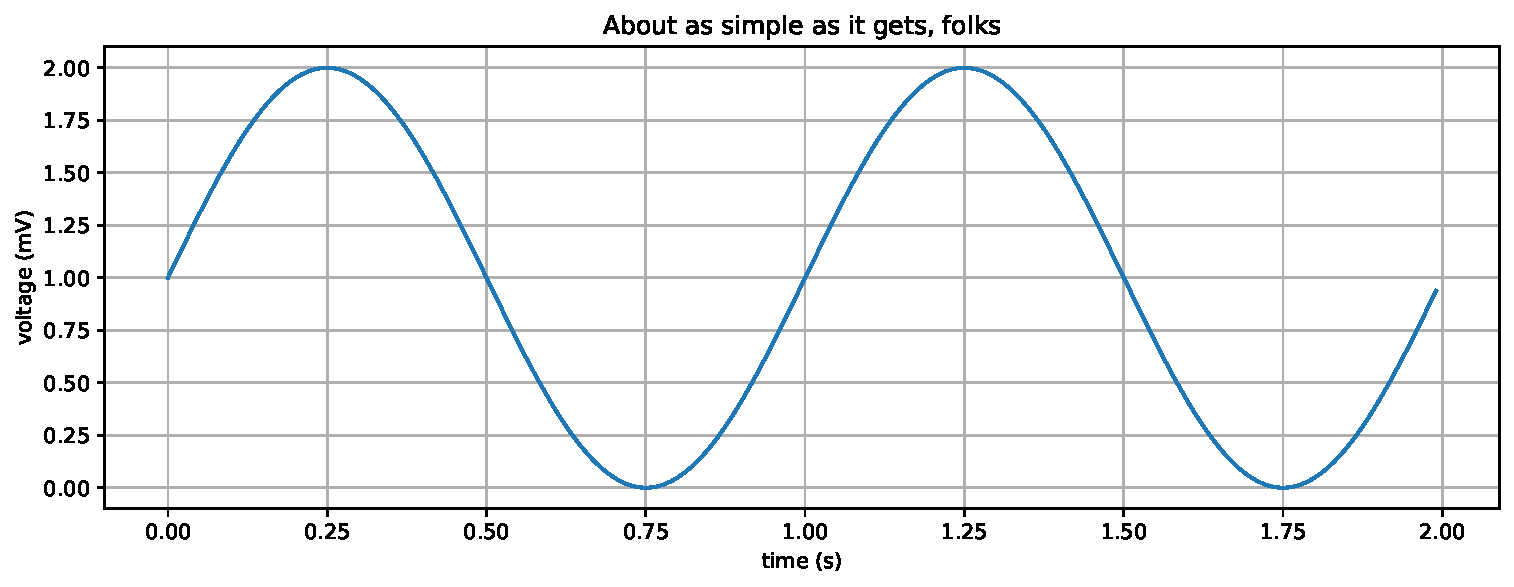
\includegraphics[width=0.8\linewidth]{test_plot.pdf}
  \caption{A sample graph}
  \label{fig:test_plot}
\end{figure}

Lots more information in this \href{https://www.latex-tutorial.com/tutorials/figures/}{tutorial}.


\section{Code Listing}
You can list code using the \emph{listings} package:

\begin{lstlisting}[language=Python,caption=Borg Pattern]
class Borg(object):
    __shared_state = {}

    def __init__(self):
        self.__dict__ = self.__shared_state
        self.state = 'Init'

    def __str__(self):
        return self.state
\end{lstlisting}

Lots more examples \href{https://www.overleaf.com/learn/latex/Code_listing}{here}.

\section{Math}
Here \ref{eq:limit} is an example of including an equation
\begin{equation}
\lim_{x\to\infty} f(x)
\label{eq:limit}
\end{equation}

More examples \href{https://www.latex-tutorial.com/tutorials/amsmath/}{here} and \href{https://www.overleaf.com/learn/latex/Mathematical_expressions}{here}.



\section{References}
Look up the bibtex references on google scholar or import from Mendeley or other reference managers. Add the bibtex snippet to the \emph{references.bib} file. Then cite the reference like this:

As explained in \cite{knuth2014art}, we also find that...

Lots more details \href{https://www.latex-tutorial.com/tutorials/bibtex/}{here}.


%%%%%%%%%%%%%%%%%%%%%%
%%% Acknowledgements
\chapter*{Acknowledgements}
In your Acknowledgements section, give credit to all the people who helped you in your project.


%%%% ADD YOUR BIBLIOGRAPHY HERE
\printbibliography

%%%%
%%%% maybe code listing here?

%%%%
\end{document}
%\end{article}
